
\documentclass[
	% -- opções da classe memoir --
	12pt,				% tamanho da fonte
	% openright,			% capítulos começam em pág ímpar (insere página vazia caso preciso)
    oneside,			% para impressão somente frente. Oposto a twoside (frente e verso)
	a4paper,			% tamanho do papel. 
	% -- opções da classe abntex2 --
	%chapter=TITLE,		% títulos de capítulos convertidos em letras maiúsculas
	%section=TITLE,		% títulos de seções convertidos em letras maiúsculas
	%subsection=TITLE,	% títulos de subseções convertidos em letras maiúsculas
	%subsubsection=TITLE,% títulos de subsubseções convertidos em letras maiúsculas
	% -- opções do pacote babel --
	english,			% idioma adicional para hifenização
	french,				% idioma adicional para hifenização
	spanish,			% idioma adicional para hifenização
	brazil,				% o último idioma é o principal do documento
	]{abntex2}


% ---
% PACOTES
% ---

% ---
% Pacotes fundamentais 
% ---
\usepackage{cmap}				% Mapear caracteres especiais no PDF
\usepackage{lmodern}			% Usa a fonte Latin Modern
\usepackage[T1]{fontenc}		% Selecao de codigos de fonte.
\usepackage[utf8]{inputenc}		% Codificacao do documento (conversão automática dos acentos)
\usepackage{indentfirst}		% Indenta o primeiro parágrafo de cada seção.
\usepackage{color}				% Controle das cores
\usepackage{graphicx}			% Inclusão de gráficos
% ---
\usepackage{float}

% ---
% Pacotes adicionais, usados no anexo do modelo de folha de identificação
% ---
\usepackage{multicol}
\usepackage{multirow}
% ---



% ---
% Pacotes adicionais, usados apenas no âmbito do Modelo Canônico do abnteX2
% ---
\usepackage{lipsum}				% para geração de dummy text
% ---

% ---
% Pacotes de citações
% ---
\usepackage[brazilian,hyperpageref]{backref}	 % Paginas com as citações na bibl
\usepackage[alf]{abntex2cite}	% Citações padrão ABNT

% --- 
% CONFIGURAÇÕES DE PACOTES
% --- 

% ---
% Configurações do pacote backref
% Usado sem a opção hyperpageref de backref
\renewcommand{\backrefpagesname}{Citado na(s) página(s):~}
% Texto padrão antes do número das páginas
\renewcommand{\backref}{}
% Define os textos da citação
\renewcommand*{\backrefalt}[4]{
	\ifcase #1 %
		Nenhuma citação no texto.%
	\or
		Citado na página #2.%
	\else
		Citado #1 vezes nas páginas #2.%
	\fi}%
% ---

% ---
% Informações de dados para CAPA e FOLHA DE ROSTO
% ---
\titulo{Documento de Especificação de Requisitos de Software: Médida Protetiva Online}
\autor{Rafael Gonçalves de Oliveira Viana}
\local{Brasil}
\data{14 de junho de 2017}
\instituicao{%
  Universidade Federal do Mato Grosso do Sul
  \par
  Câmpus Coxim
  \par
  Sistema de Informação}
\tipotrabalho{Documento de Especificação de Requisitos de Software}
% O preambulo deve conter o tipo do trabalho, o objetivo, 
% o nome da instituição e a área de concentração 
\preambulo{Levantamento de requisitos, referente ao trabalho I, realizado na matéria de Engenharia Web I, ministrada pelo M. Prof. Marcel Seiji Kay}
% ---

% ---
% Configurações de aparência do PDF final

% alterando o aspecto da cor azul
\definecolor{blue}{RGB}{41,5,195}

% informações do PDF
\makeatletter
\hypersetup{
     	%pagebackref=true,
		pdftitle={\@title}, 
		pdfauthor={\@author},
    	pdfsubject={\imprimirpreambulo},
	    pdfcreator={LaTeX with abnTeX2},
		pdfkeywords={abnt}{latex}{abntex}{abntex2}{relatório técnico}, 
		colorlinks=true,       		% false: boxed links; true: colored links
    	linkcolor=blue,          	% color of internal links
    	citecolor=blue,        		% color of links to bibliography
    	filecolor=magenta,      		% color of file links
		urlcolor=blue,
		bookmarksdepth=4
}
\makeatother
% --- 

% --- 
% Espaçamentos entre linhas e parágrafos 
% --- 

% O tamanho do parágrafo é dado por:
\setlength{\parindent}{1.3cm}

% Controle do espaçamento entre um parágrafo e outro:
\setlength{\parskip}{0.2cm}  % tente também \onelineskip

% ---
% compila o indice
% ---
\makeindex
% ---

% ----
% Início do documento
% ----
\begin{document}
% Retira espaço extra obsoleto entre as frases.
\frenchspacing 

% ----------------------------------------------------------
% ELEMENTOS PRÉ-TEXTUAIS
% ----------------------------------------------------------

\imprimircapa

\imprimirfolhaderosto*

\tableofcontents
% ----------------------------------------------------------
% ELEMENTOS TEXTUAIS  (necessário para incluir número nas páginas)

% ----------------------------------------------------------

\textual



% ----------------------------------------------------------
% Introdução
% ----------------------------------------------------------

\chapter{Documento de Requisitos} %% NOVO CAPÍTULO (REPARE QUE ELE AUTOMATICAMENTE JÁ COLOCA O NÚMERO DO CAPÍTULO E JÁ ADICIONA NO SUMÁRIO)
	\section{Descrição do Sistema}
		O sistema para Poíicia Militar consiste em desenvolver um gerenciador de medidas protetivas, expedida pela Justiça. Cada medida tem uma ou mais vitimas e um ou mais Réus, contendo data de emissão, observação e um valor em dias que representa quantos dias esta em vigor essa medida. Com a medida já em mão deve-se cadastradcla colocando esses dados para possível consulta de uma versão previamente digitalizada, assim como criar relatórios online.
	
		O sifdsastema deve ainda emitir diversos tipos de relatórios e consultas, possibilitando um melhor gerenciamento do policiamento ostencivo economisando recursos para melhores aplicações.
		
	\section{Objetivos do documento}
	
		Este documento tem o objetivo de definir os requisitos do sistema medida protetiva. Nele estão contemplados os requisitos funcionais e não-funcionais, casos de uso e regras de negócio do sistema.
	
	\section{Escopo do documento}
	
		Este documento define os requisitos funcionais e não funcionais casos de uso e regras de negócios correlatos para o sistema acima citado. Para elucidação de termos específicos utilizados neste documento, faz-se necessária referência ao Glossário.

	\section {Requisitos Funcionais}\label{RF}
	
		\subsection{Login (Usuário/Gerenciador)}\label{RF1}
			\begin{enumerate}
				\item O sistema deve possuir 2 niveis de usuários com diferentes privilégios no sistma sendo eles: gerenciador e usuário.\label{login1}
				 \item O gerenciador abastecer o sistema podendo consultar e imprimir relatórios.
				 \item O usuário apenas consulta e imprimi relatórios.
			
			\end{enumerate}
		 
		\subsection{Lançamentos das medidas protetivas}\label{RF2} 
	    	\begin{enumerate} 
				\item O sistema deve permitir que apenas o usuário gerenciador realize a inclusão, alteração e remoção de medidas protetivas scaneadas em PDF e anexadas, juntamente do cadastro individual contendo os seguintes atributos: nome, endereço, cidade onde mora, estado, país, telefone, documento de identificação (RG ou CPF para brasileiros e passaporte para estrangeiros), data de nascimento e nome dos pais(“se constar na medida”) de ambas as vitimas e acusados, que constam na médida protetiva.\label{teste}
			
		   	\end{enumerate}
   	
		\subsection{Impressão de relatórios e consultas}\label{RF3}
			\begin{enumerate}
				\item O sistema deve criar relatórios e gráficos de bairro, cidades, vitimas e acusados com maiores e menores índices de medidas protetivas, cada relatório deve ser individual para cada uma das opções citadas acima, os dois niveis de usuários poderam acessar essa opção.
				\item O sistema deve permitir a consulta de uma medida protetiva online, pelo nome da vítima, nome do acusado ou pelo cpf dos mesmos, tento acesso ao documento original scaneado e armazenado online.
			\end{enumerate}
	

	\section{Requisitos não funcionais}
	
		\subsection{Confiabilidade} \label{sec:RFN01}
			\begin{enumerate}
				\item O sistema deve ter capacidade para recuperar os dados perdidos da última operação que realizou em caso de falha.
				\item O sistema deve fornecer ferramentas para a realização de backups dos arquivos do sistema.
				\item O sistema deve possuir senhas de acesso e identificação para diferentes tipos de usuários: usuário e gerenciador.
			\end{enumerate}

	
		\subsection{Eficiência}\label{sec:RFN02}
			\begin{enumerate}
				\item O sistema deve responder a consultas on-line em menos de 5 segundos.
				\item O sistema deve iniciar a impressão de relatórios solicitados dentro de no máximo 20 segundos após sua requisição.
			\end{enumerate}
		\subsection{Portabilidade}\label{sec:RFN03}
			\begin{enumerate}
				\item O sistema deve ser web e adaptavel para dispositivos moveis.
			\end{enumerate}
		\subsection{Disponibilidade}\label{sec:RFN04}
			\begin{enumerate}
				\item O sistema deve estar 24 horas nos 7 dias da semenana online.
			\end{enumerate}
%\chapter{Caso de Uso}		
	\section{Lista de Casos de Uso}
		Alguns dos casos de uso necessários para a implementação do sistema estão listados nesta seção:
		\begin{enumerate}
			\item Cadastro de Atores no sistema. \label{Lista:1}
			\item Login de Atores no Sistema.\label{Lista:2}
			\item Cadastro de Medida Protetiva no sistema.\label{Lista:3}
			\item Consulta de Medida Protetiva no sistema.\label{Lista:4}
			\item Editar Medida Protetiva do sistema.\label{Lista:5}
			\item Excluir Medida Protetiva do sistema.\label{Lista:6}
		\end{enumerate}
	\section{Mapeamento de caso de uso}
		 Nesta seção os requisitos funcionais (RF) serão mapeados em casos de uso. Os casos de uso que serão implementados, estarão descritos detalhadamente na seção \ref{RF}.

		\begin{center}
			\begin{tabular}{ |c|c|c|c| } 
				\hline
				Requisitos funcionais
				RF  & Casos de uso envolvidos
				CU \\
				\hline
				~RF \ref{RF1} & \ref{Lista:1} e \ref{Lista:2} \\ 
				\hline
				~RF \ref{RF2}  e~RF  \ref{RF3} & \ref{Lista:3}, \ref{Lista:4}, \ref{Lista:5} e \ref{Lista:6}   \\ 
				\hline
			
			\end{tabular}
		\end{center}
	
	   \subsection{Caso de uso cadastro}\label{CU:01}
		\begin{table}[H]
			\caption{Caso de Uso de Cadastro}
			\centering
			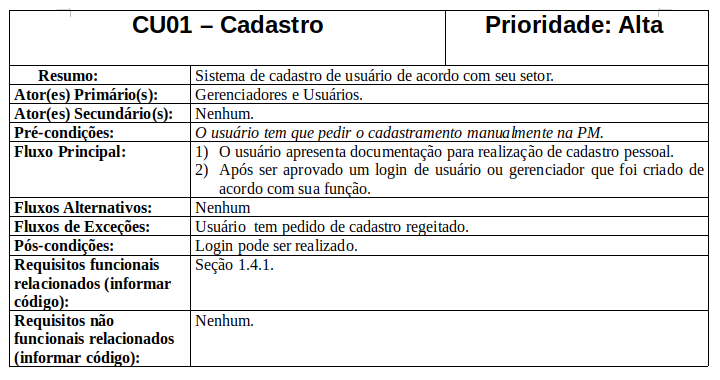
\includegraphics[width=0.5\textheight]{CU01.png}
		\end{table}
		\begin{figure}[H]
			\caption{Caso de Uso de Cadastro}
			\centering
			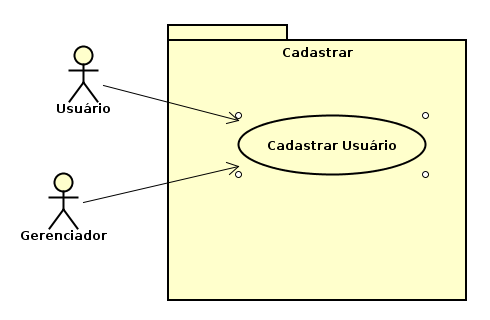
\includegraphics[width=0.5\textheight]{Cadastro.png}
		\end{figure}
		\subsection{Caso de uso login}\label{CU:02}
		\begin{table}[H]
			\caption{Caso de Uso de Login}
			\centering
			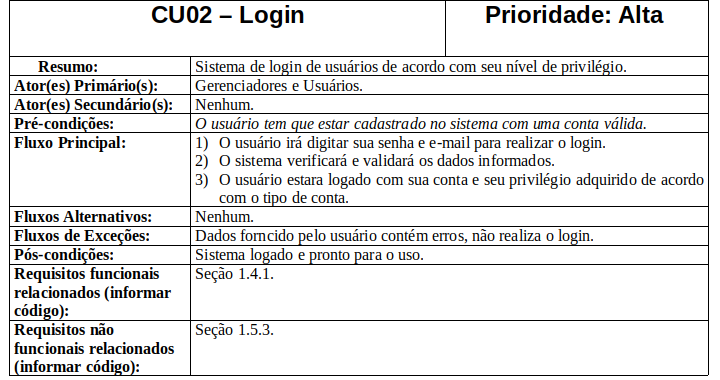
\includegraphics[width=0.5\textheight]{CU02.png}
		\end{table}
		\begin{figure}[H]
			\caption{Caso de Uso de Login}
			\centering
			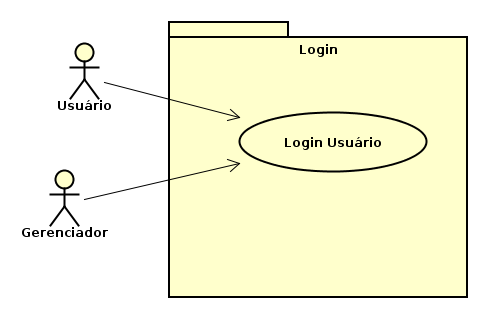
\includegraphics[width=0.5\textheight]{Login.png}
		\end{figure}
		\subsection{Caso de uso gerenciador} \label{CU:03}
		\begin{table}[H]
			\caption{Caso de Uso de Gerenciador}
			\centering
			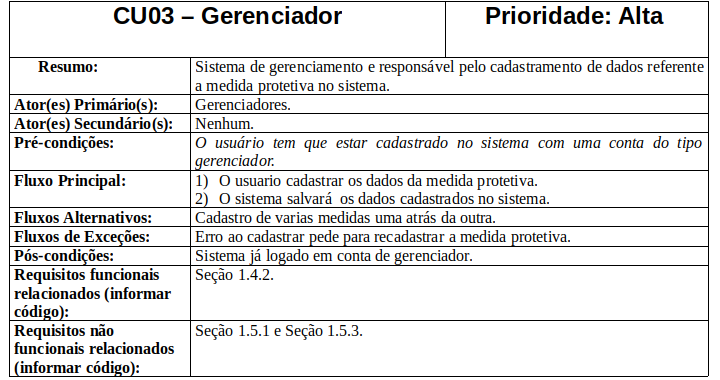
\includegraphics[width=0.5\textheight]{CU03.png}
		\end{table}
		\begin{figure}[H]
			\caption{Caso de Uso de Gerenciador}
			\centering
			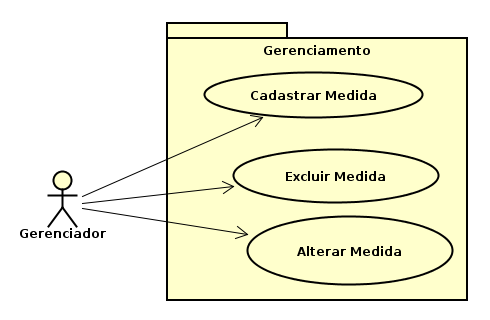
\includegraphics[width=0.5\textheight]{Gerenciamento.png}
		\end{figure}
		\subsection{Caso de uso consultas e relatórios}\label{CU:04}
		\begin{table}[H]
			\caption{Caso de Uso de Consultas e Relatórios}
			\centering
			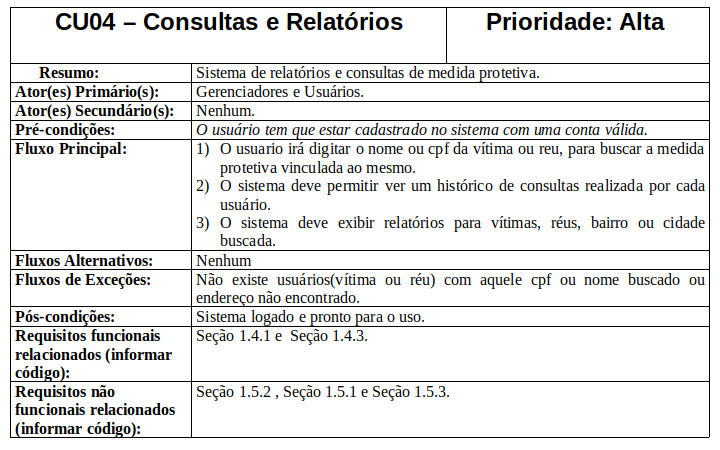
\includegraphics[width=0.5\textheight]{CU04.png}
		\end{table}
		\begin{figure}[H]
			\caption{Caso de Uso de Consultas e Relatórios}
			\centering
			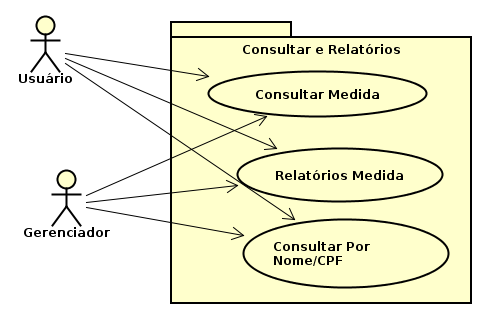
\includegraphics[width=0.5\textheight]{Consulta-Relatorio.png}
		\end{figure}
	

		
	\section{Lista de Regras de negócio}
		\begin{enumerate}
			\item Os gerenciadores só serão aceitos se forem da P2(Setor responsável pela medida protetiva na PM-MS).\label{LISTAN:01}
			\item As atualizações referente a medida protetiva só serão realizadas das 08:00 às 13:30 de Segunda à Sexta feira.\label{LISTAN:02}
		\end{enumerate}
	
	
	\section{Mapeamento de regras de negócio}	
		 Nesta seção as regras de negócio (RN) serão mapeadas em casos de uso. Os casos de uso que serão implementados, estarão descritos detalhadamente na seção \ref{RF}.
	
		\begin{center}
			\begin{tabular}{ |c|c|c|c| } 
				\hline
				Regras de Negócio
				RN  & Casos de uso envolvidos
				CU \\
				\hline
				~RN \ref{LISTAN:01}  &  CU \ref{CU:03}  \\ 
				\hline
				
			\end{tabular}
		\end{center}
		\subsection{Setor resposável}
			\begin{center}
			
					\begin{tabular}{|l|}
						\hline
						Casos de uso relacionados/Origem das regras de negócio: NÃO HÁ.  
						\\ \hline
						RN \ref{LISTAN:01}: Regras de aprovação de usuário gerenciador.                                                                   \\ \hline
						Descrição: Para ser um gerenciador tem que pertencer Setor P-2. \\ \hline
						Casos de uso relacionados/Origem das regras de negócio: CU \ref{CU:03}.                                                                   \\ \hline
					\end{tabular}
			
			\end{center}
		\subsection{Abastecimento dos dados}

				\begin{center}
				
				\begin{tabular}{|l|}
					
					\hline
					Casos de uso relacionados/Origem das regras de negócio: NÃO HÁ.  
					\\ \hline
					RN \ref{LISTAN:02}: Regras do horário para abastecimento dos dados.                                                                   \\ \hline
					Descrição: Os dados somente serám abastecido  no sistema entre 07h as 14h. \\ \hline
					Casos de uso relacionados/Origem das regras de negócio: NÃO HÁ.                                                                  \\ \hline
				\end{tabular}
				
			\end{center}
			\section{Glossário}
	
				\begin{center}
				
				\begin{tabular}{|l|}
					
					\hline
			\textbf{Glossário}	  
					\\ \hline
					\textbf{Backup}: Cópia de segurança ou cópia de salvaguarda
					 .                                                                   \\ \hline
					
					\textbf{Medida Protetiva}: Uma medida protetiva e um documento                                      \\ 
					expedido pelo juiz com poder de proteção para a vitima.                           
					\\ \hline
				\end{tabular}
				
			\end{center}


% ----------------------------------------------------------
% ELEMENTOS PÓS-TEXTUAIS
% ----------------------------------------------------------
\postextual


% ----------------------------------------------------------
% Referências bibliográficas
% ----------------------------------------------------------


% ----------------------------------------------------------
% Glossário
% ----------------------------------------------------------
%
% Consulte o manual da classe abntex2 para orientações sobre o glossário.

\clearpage

% ----------------------------------------------------------
% Apêndices
% ----------------------------------------------------------

% ---
% Inicia os apêndices
% ---
\begin{apendicesenv}

% Imprime uma página indicando o início dos apêndices
\partapendices

% ----------------------------------------------------------
%\chapter{Quisque libero justo}
% ----------------------------------------------------------

%\lipsum[50]


\end{apendicesenv}
% ---


% ----------------------------------------------------------
% Anexos
% ----------------------------------------------------------

%---------------------------------------------------------------------
% INDICE REMISSIVO
%---------------------------------------------------------------------

\printindex

%---------------------------------------------------------------------
% Formulário de Identificação (opcional)
%---------------------------------------------------------------------
\chapter*[Médida Protetva]{Médida Protetva}
\addcontentsline{toc}{chapter}{Exemplo Formato Medida Protetva}
\label{formulado-identificacao}

Exemplo de medida protetiva

\bigskip

\begin{tabular}{|p{9cm}|p{5cm}|} %% EXEMPLO DE TABELA MAIS COMPLEXA
\hline
\multicolumn{2}{|c|}{\textbf{\large Médida Protetiva}}\\
\hline
\multirow{4}{10cm}[24pt]{Título e subtítulo}& Classificação de segurança\\
                   & \\
                   \cline{2-2}
                   & No.\\
                   & \\
				
\hline
Local de Expedição & Data\\

\hline
\multicolumn{2}{|l|}{Autor(es)} \\

\hline
\multicolumn{2}{|l|}{Vítimas} \\
\hline
\multicolumn{2}{|l|}{Resumo}\\[3cm]
\hline

\end{tabular}

\end{document}
